\chapter{Performance Evaluation of Machine Learning Methods}\epigraph{You want to evaluate future borrowers, but in order to train an algorithm that will help you identify future defaults, you have to train it and evaluate it on past data.}{Anthony Goldbloom}\label{Chapter:4}

Evaluating results of outlier detection algorithms and measuring their effectiveness is an essential task. The main requirement for evaluation is the availability of ground-truth about the class membership. Since the ground truth is available, a part of the data can be used for training and the remaining for evaluation. 

This chapter describe the measurement technique which is used in Chapter~\ref{Chapter:5:Results} to evaluate the experimental (classification) results. 

\section[Receiver Operating Characteristic Analysis (ROC)] {Receiver Operating Characteristic Analysis (ROC) \footnote{The terms in the scope of ROC analysis can vary (e.g true positive rate = hit rate ...), for the sake of consistency the below explanation will follow notation in  \cite{Fawcett:2006:IRA:1159473.1159475}}.}\label{Chapter:4:ROC}

ROC analysis is a technique to measure and visualize the performance of a classifier through calculating the tradeoff between hit rates and false alarms \cite{Fawcett:2006:IRA:1159473.1159475}. This performance evaluation technique is mostly applied to binary classifiers.

Regardless of a classifier, there are four types of a prediction outcome, covering all possible scenarios:

\begin{itemize}
    \item \textbf{True Positive (TP): }  If an instance is positive and it was classified as positive.
      \item \textbf{False Positive (FP): } If an instance is negative and it was classified as positive.
    \item \textbf{True Negative (TN):}  If an instance is negative and it was classified as negative.
    \item \textbf{False Negative (FN):}  If an instance is positive and it was classified as negative.
\end{itemize}

It is common practice to construct a \textit{confusion matrix} (see Figure~\ref{fig:confusion-matrix}) to combine these four characteristics. Along the main diagonal correct decisions are given where the errors (confusion) are represented along the minor diagonal of the matrix (see Figure~\ref{fig:confusion-matrix}).

\begin{figure}[h!]
    \centering
    \fbox{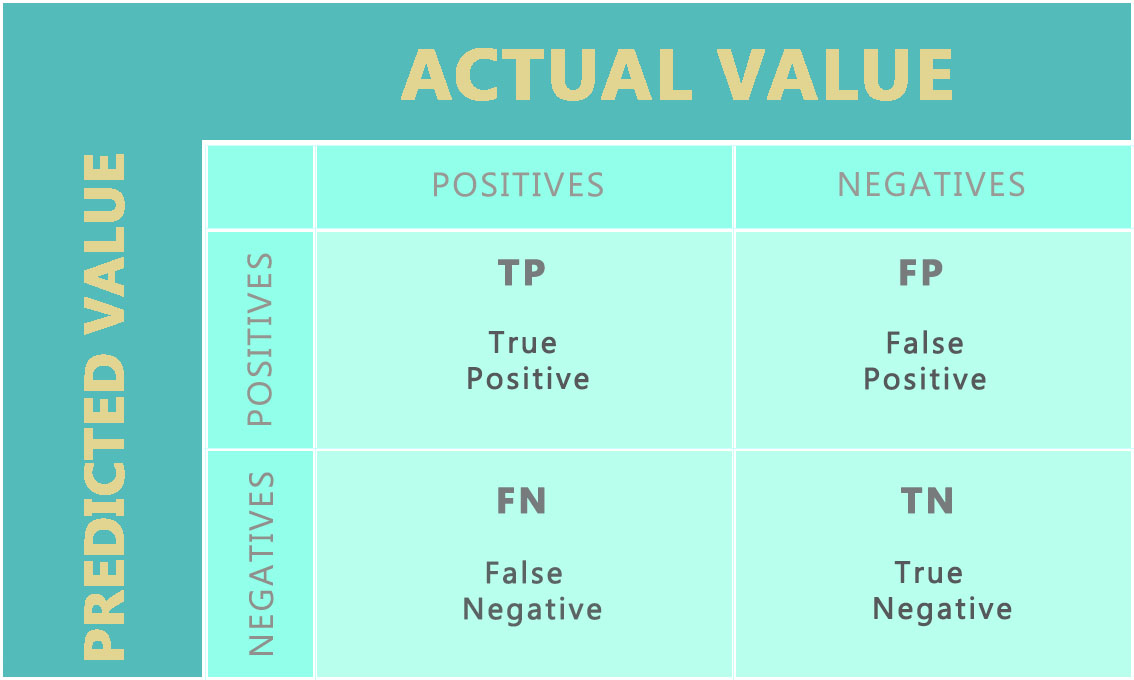
\includegraphics[scale=0.25]{Graphics/confusion-matrix.png}}
    \caption{Confusion Matrix.}
    \label{fig:confusion-matrix}
\end{figure}

Based on the above given types of predictions, additional measures can be calculated, such as:

\[ \textrm{False Positive Rate (FP-Rate)} = \frac{FP}{N}, \textrm{where } N \textrm{ stands for negatives.}  \]
\[ \textrm{True Positive Rate (TP-Rate)} = \frac{TP}{P}, \textrm{where } P \textrm{ stands for positives.}  \]


A discrete classifier have by definition a class label as output instead of probability (e.g \(Y\)/\(N\) for binary classification) \cite{Fawcett:2006:IRA:1159473.1159475}. The results can be easily  represented on a basic ROC-Graph (see Figure~\ref{fig:roc-graph}), where the \(x\) - axis is the FP-Rate and \(y\) is the TP-Rate. The best classifier/point on the graph is the one with the highest true positive and the lowest false positive rate (point \(D\) in Figure~\ref{fig:roc-graph}).
\begin{figure}
\centering
\begin{minipage}{.5\textwidth}
  \centering
  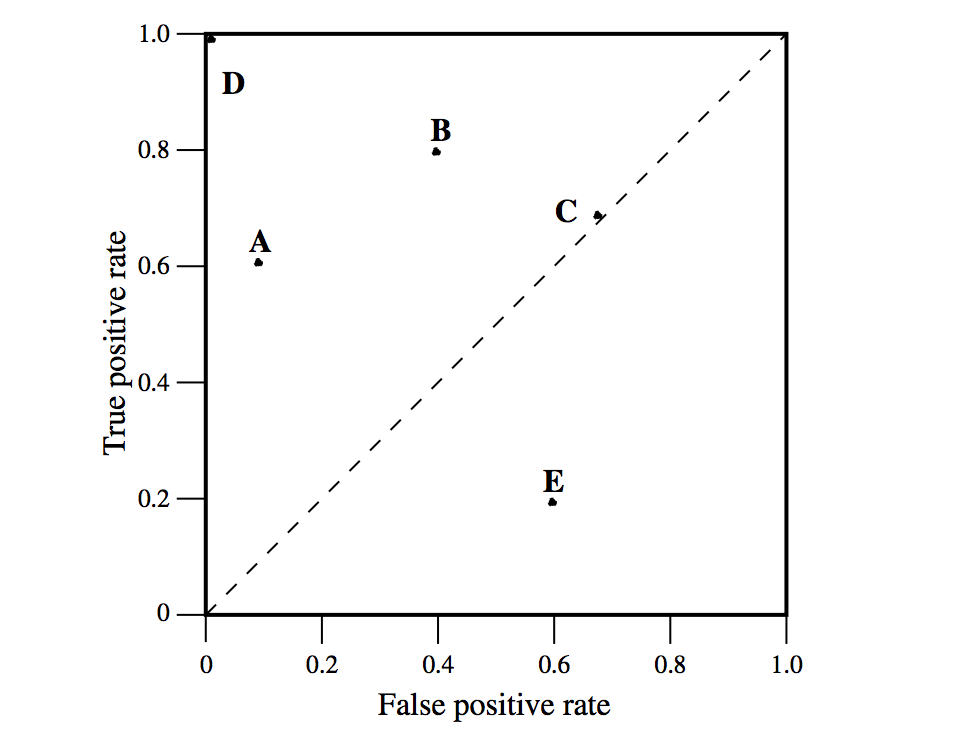
\includegraphics[scale=0.47]{Graphics/roc-graph.png}
  \captionof{figure}{ROC-Graph for a discrete classifier. From: \textit{Figure is taken from the work of~\cite{Fawcett:2006:IRA:1159473.1159475}}}
  \label{fig:roc-graph}
\end{minipage}%
\begin{minipage}{.5\textwidth}
  \centering
    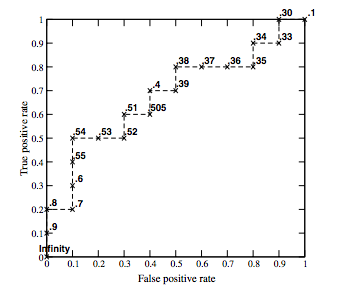
\includegraphics[scale=0.57]{Graphics/roc-curve.png}
  \captionof{figure}{ROC-Curve for a probabilistic classifier. From: \textit{Figure is taken from the work of~\cite{Fawcett:2006:IRA:1159473.1159475}}}
  \label{fig:roc-curve}
\end{minipage}
\end{figure}
An also interesting observation is the \(C\), located on the diagonal dotted line, where the FP and TP rates are equal for any pair of rates. The dotted line corresponds to a random classifier, which implies that for any classifier to be better than random, its point related to the ROC-Graph should be located above the dotted line.

Some classifiers yields numeric (real) values as an output. These values are either strict probabilities or they can be uncalibrated scores that may be turned into probability. These values can be converted into binary labels by using a threshold, e.g., if the value is above the threshold then the label is \(Y\) else \(N\). So, each threshold would produce a different point in ROC space, and connecting the points together produces the ROC-Curve (see Figure~\ref{fig:roc-curve}). 

ROC analysis is thus a useful tool for measuring classifier performance. Whenever a discrete classifier is used yielding crisp labels, a confusion matrix provides an additional view on classifier performance that complements a ROC-Graph. With a classifier capable of calculating the probabilities, a ROC-Curve is a natural choice for performance evalution. For imbalanced data sets like the one used in this thesis, the ROC analysis results in unbiased performance evaluation that is not influenced (dominated) by a majority class, in contrast to such measures as classification accuracy  \cite{Fawcett:2006:IRA:1159473.1159475}.

 


%Another important property of ROC-Curve it is slightly sensitive to the distribution of particular classes in the data (e.g the proportions of FP-Rate <-> TP-Rate). This may an attractive feature if true negative is not much valuable to the problem, or negative examples are abundant but in the case of a fraud detection problem, where negative (fraud) examples are by definition rare, the ROC-Graph will not provide enough insides to measure classification right caused by skewed class distribution. Thus, additional metrics required.


%Bellow, precision, and recall are given, both of them are sensitive to the class distribution due to the fact that the calculation is also related to the opposite classification category (TP-Rate is related to True Positives and the amount of positives where precision also include false negatives in the calculation):

%\[ \textrm{Positive precision  (precision)} = \frac{TP}{TP+FN}  \]
%\[ \textrm{Negative recall (recall)} = \frac{TN}{TN+FP}  \]

%An example in figure\footnote{Figure is taken from the work of \cite{Fawcett:2006:IRA:1159473.1159475}} \ref{fig:roc-pr-curve} illustrate classification on two data sets differ by the amount of negatives. The curves on (a) and (c) (ROC-Curve) show up only a minimal change although a number of negatives is differed by 10 times, where the positive-recall graph on (b) and (d) differ substantially. 

%\begin{figure}[h!]
    %\centering
    %\includegraphics[scale=0.8]{Graphics/curves-vs-pr%-analysis.png}
%    \caption{ROC-Curve for probabilistic classifier.}
%    \label{fig:roc-pr-curve}
%\end{figure}


